\section{圆的基本概念}

\begin{theorem}[两点间的距离公式]
    设点 $A(x_1,y_1)$ 和点 $B(x_2,y_2)$ ，则两点间的距离 $d$ 为
    \[
        d = \sqrt{(x_2-x_1)^2+(y_2-y_1)^2}.
    \]

    该公式可以通过勾股定理推导得到。

    \begin{figure}[H]
        \centering
        \resizebox{0.3\textwidth}{!}{%
            \begin{circuitikz}
                \tikzstyle{every node}=[font=\normalsize]
                \draw [->, >=Stealth] (5.5,9.25) -- (13.25,9.25);
                \node [font=\normalsize] at (10,10) {$\triangle x = x_1-x_2$};
                \draw [->, >=Stealth] (7,7.75) -- (7,14.25);
                \draw [short] (8,10.5) -- (11.75,13.5);
                \draw [short] (11.75,13.5) -- (11.75,10.5);
                \draw [short] (11.75,10.5) -- (8,10.5);
                \draw [<->, >=Stealth] (8,10.25) -- (11.75,10.25);
                \draw [<->, >=Stealth] (12,13.5) -- (12,10.5);
                \node [font=\normalsize, rotate around={-90:(0,0)}] at (12.5,12) {$\triangle y = y_1-y_2$};
                \draw [short] (11.5,10.5) -- (11.5,10.75);
                \draw [short] (11.5,10.75) -- (11.75,10.75);
                \node [font=\normalsize] at (7.75,11) {$A(x_1,y_1)$};
                \node [font=\normalsize] at (11.75,13.75) {$B(x_2,y_2)$};
            \end{circuitikz}
        }%
        \label{fig:my_label}
    \end{figure}
\end{theorem}

\begin{definition}[圆的标准方程]
    因为能一眼看出圆的圆心和半径，所以圆的标准方程为 $(x-a)^2+(y-b)^2=r^2$，其中 $(a,b)$ 是圆心，$r$ 是半径。

    \begin{center}
        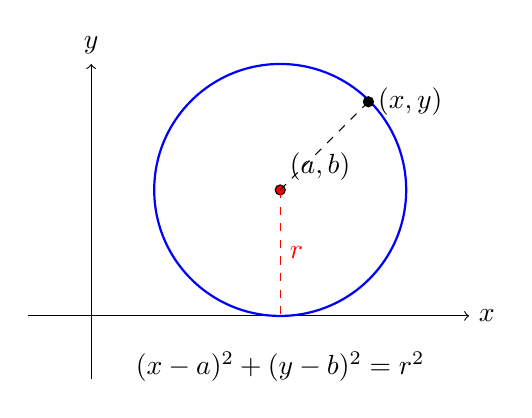
\begin{tikzpicture}[scale=0.8]
            % 绘制坐标轴
            \draw[->] (-1,0) -- (6,0) node[right] {$x$};
            \draw[->] (0,-1) -- (0,4) node[above] {$y$};

            % 绘制圆
            \draw[thick, blue] (3,2) circle (2);

            % 标记圆心和半径
            \draw[fill=red] (3,2) circle (0.08) node[above right] {$(a,b)$};
            \draw[dashed, red] (3,2) -- (3,0) node[midway, right] {$r$};

            % 标记一个圆上的点
            \draw[fill=black] (4.4,3.4) circle (0.08) node[right] {$(x,y)$};
            \draw[dashed] (3,2) -- (4.4,3.4);

            % 添加方程说明
            \node at (3,-0.8) {$(x-a)^2+(y-b)^2=r^2$};
        \end{tikzpicture}
    \end{center}
\end{definition}

\begin{example}
    求解下列圆的圆心和半径
    \begin{itemize}
        \item 求 $(x+2)^2+(y-\sqrt{ln2})^2=e^9$ 的圆心和半径
        \item 求 $(x-\sqrt{3}-1)^2+(y+2)^2=18$ 的圆心和半径。
    \end{itemize}

\end{example}

\v{4em}

\begin{example}
    动点 $A$ 在圆 $C: x^2+y^2-6 x-8 y+21=0$ 上运动，则点 $A$ 到 $x$ 轴的最近距离是 \underline{\qquad}
\end{example}

\begin{definition}[圆的一般方程]
    圆的一般方程为 $x^2+y^2+Dx+Ey+F=0$，其中 $D$，$E$，$F$ 是常数。

    将一般方程变形为标准方程：
    \begin{align}
        x^2+y^2+Dx+Ey+F                                                       & = 0                              \\
        \left(x^2+Dx+\frac{D^2}{4}\right) + \left(y^2+Ey+\frac{E^2}{4}\right) & = -F+\frac{D^2}{4}+\frac{E^2}{4} \\
        \left(x+\frac{D}{2}\right)^2 + \left(y+\frac{E}{2}\right)^2           & = \frac{D^2+E^2-4F}{4}
    \end{align}

    因此，圆心坐标为 $\left(-\frac{D}{2}, -\frac{E}{2}\right)$，半径为 $r = \frac{\sqrt{D^2+E^2-4F}}{2}$。
\end{definition}

\begin{example}
    设 $a \in \mathbf{R}$ ．已知方程 $x^2+y^2-4 x+a=0$ 表示的曲线是一个圆，则 $a$ 的取值范围为 \underline{\qquad}
\end{example}

\v{6em}

\begin{example}
    实数 $a>0$ ，圆 $C: x^2+y^2-4 x+a y=0$ 的面积为 $8 \pi$ ，则 $a=$ \underline{\qquad}
\end{example}

\begin{theorem}[圆的判别式定理]
    \begin{minipage}[c]{0.5\textwidth}
        对于一般方程 $x^2+y^2+Dx+Ey+F=0$ 表示的图形：
        \begin{itemize}
            \item 当 $D^2+E^2-4F > 0$ 时，表示一个圆
            \item 当 $D^2+E^2-4F = 0$ 时，表示一个点
            \item 当 $D^2+E^2-4F < 0$ 时，不表示任何实数解的图形
        \end{itemize}

        判别式 $\Delta = D^2+E^2-4F$ 可判断其几何意义。
    \end{minipage}
    \begin{minipage}[c]{0.5\textwidth}
        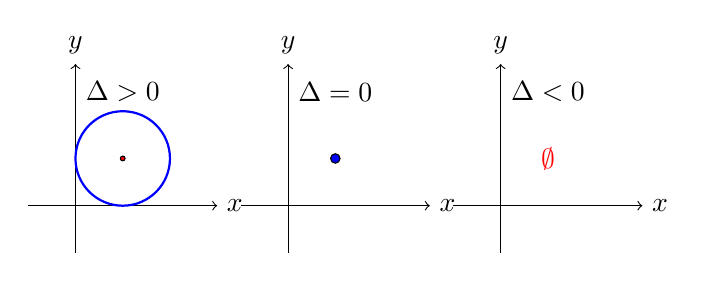
\begin{tikzpicture}[scale=0.6]
            % 第一个图：圆
            \begin{scope}[xshift=0cm]
                \draw[->] (-1,0) -- (3,0) node[right] {$x$};
                \draw[->] (0,-1) -- (0,3) node[above] {$y$};
                \draw[thick, blue] (1,1) circle (1);
                \draw[fill=red] (1,1) circle (0.05);
                \node[above] at (1,2) {$\Delta > 0$};
            \end{scope}

            % 第二个图：点
            \begin{scope}[xshift=4.5cm]
                \draw[->] (-1,0) -- (3,0) node[right] {$x$};
                \draw[->] (0,-1) -- (0,3) node[above] {$y$};
                \draw[fill=blue] (1,1) circle (0.1);
                \node[above] at (1,2) {$\Delta = 0$};
            \end{scope}

            % 第三个图：无实数解
            \begin{scope}[xshift=9cm]
                \draw[->] (-1,0) -- (3,0) node[right] {$x$};
                \draw[->] (0,-1) -- (0,3) node[above] {$y$};
                \node[red] at (1,1) {$\emptyset$};
                \node[above] at (1,2) {$\Delta < 0$};
            \end{scope}
        \end{tikzpicture}
    \end{minipage}
\end{theorem}

\begin{example}
    下列方程一定表示圆的是 （其中 $a, b \in \mathbf{R}$）（\qquad）
    \begin{tasks}(4)
        \task $x^2+y^2=0$
        \task $x^2+y^2-2 x+4 y-6=0$
        \task $x^2+y^2+2 a x-b^2=0$
        \task $x^2+2 x y+y^2-9=0$
    \end{tasks}
\end{example}

\v{8em}

\subsection{已知三点求圆的方程}

\begin{theorem}
    \begin{itemize}
        \item 可以构造两条直线相交来求解。
        \item 使用一般式构造三元方程求解更快。
    \end{itemize}
\end{theorem}

\begin{example}
    $\triangle A B C$ 的三个顶点分别是 $A(4,0)$、$B(0,2)$ 、$C(3,1)$ ．
    \begin{enumerate}
        \item 求 $\triangle A B C$ 的外接圆 $G$（ $G$ 为圆心）的标准方程．
    \end{enumerate}
\end{example}

\begin{solution}
    设圆 $G$ 的方程为 $x^2+y^2+D x+E y+F=0$（其中 $D^2+E^2-4 F>0$ ）

    因为 $A$、$B$、$C$ 三点都在圆上，可得 $\left\{\begin{array}{l}4 D+F+16=0 \\ 2 E+F+4=0 \\ 3 D+E+F+10=0\end{array}\right.$

    解得 $D=0, ~ E=6, ~ F=-16$ ，满足 $D^2+E^2-4 F>0$

    所以所求圆 $G$ 的方程为 $x^2+y^2+6 y-16=0$ ，即 $x^2+(y+3)^2=25$ ．
\end{solution}

\v{2em}

\begin{example}
    在平面直角坐标系中．求经过三点 $(0,0),(1,1),(2,0)$ 的圆的方程（通过画图可以简单解决）
\end{example}

\v{12em}

\begin{example}
    在平面直角坐标系中，曲线 $y=x^2-4 x+3$ 与坐标轴的公共点都在圆 $C$ 上，求圆 $C$ 的标准方程；
\end{example}

\v{12em}

\subsection{已知过两点求圆的方程}

\begin{example}
    已知圆 $C$ 的圆心在直线 $2 x-y-5=0$ 上，且经过点 $A(0,3), ~ B(4,-1)$ ．
    \begin{enumerate}
        \item 求圆 $C$ 的标准方程；
        \item 求过原点且与圆 $C$ 相切的直线方程
    \end{enumerate}
\end{example}

\v{12em}

\begin{example}
    已知圆 $C$ 经过 $P(-2,4), ~ Q(3,-1)$ 两点，且在 $x$ 轴上截得的弦长等于 6 ，则圆 $C$ 的一般方程为 \underline{\qquad}
\end{example}

\begin{solution}
    设圆 $C$ 的方程为 $x^2+y^2+D x+E y+F=0$ ．

    由题意可得 $\left\{\begin{array}{c}2 D-4 E-F=20 \\ 3 D-E+F=-10\end{array}\right.$ ，

    在圆 $C$ 的方程中，令 $y=0$ ，得 $x^2+D x+F=0$ ．（2）

    设 $x_1$ ，$x_2$ 是方程（2）的两根，由 $\left|x_1-x_2\right|=6$ ，得 $D^2-4 F=36$ ，（3）

    联立（1）（3）得 $D=-2, E=-4, F=-8$ 或 $D=-6, E=-8, F=0$ ．

    故圆 $C$ 的一般方程为 $x^2+y^2-2 x-4 y-8=0$ 或 $x^2+y^2-6 x-8 y=0$ ．
\end{solution}

\begin{example}
    已知圆 $C$ 经过 $P(2,-2), ~ Q(0,-2)$ 两点，且在 $y$ 轴上截得的弦长等于 4 ，则圆 $C$ 的一般方程为 \underline{\qquad\qquad}
\end{example}

\begin{solution}
    设圆 $C$ 的方程为 $x^2+y^2+D x+E y+F=0$ ．

    由题意，将 $P(2,-2), ~ Q(0,-2)$ 代入圆的方程可得：
    $\left\{\begin{array}{l} 4+4+2D-2E+F=0 \\ 0+4+0D-2E+F=0 \end{array}\right.$
    即 $\left\{\begin{array}{l} 2D - 2E + F = -8 \\ -2E + F = -4 \end{array}\right.$ (1)

    在圆 $C$ 的方程中，令 $x=0$ ，得 $y^2+E y+F=0$ ．（2）

    设 $y_1$ ，$y_2$ 是方程（2）的两根，代表圆与 $y$ 轴的两个交点的纵坐标。

    可知 $|y_1-y_2| = \sqrt{(y_1+y_2)^2-4y_1y_2} = \sqrt{(-E)^2-4F} = \sqrt{E^2-4F}$．

    因为在 $y$ 轴上截得的弦长等于 4 ，所以 $E^2-4 F=16$ ．（3）
\end{solution}

\v{12em}

\subsection{点和圆的位置关系}

\begin{theorem}[点和圆的位置关系]
    \begin{minipage}[c]{0.5\textwidth}
        比较点到圆心的距离与半径的大小：
        \begin{itemize}
            \item 点在圆内部：$(x_0-a)^2+(y_0-b)^2 < r^2$
            \item 点在圆外部：$(x_0-a)^2+(y_0-b)^2 > r^2$
            \item 点在圆上：$(x_0-a)^2+(y_0-b)^2 = r^2$
        \end{itemize}
        可判断点和圆的位置关系。
    \end{minipage}
    \begin{minipage}[c]{0.5\textwidth}
        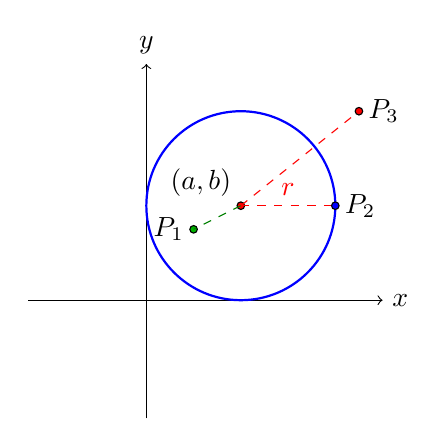
\begin{tikzpicture}[scale=0.6]
            % 绘制坐标轴
            \draw[->] (-2.5,0) -- (5,0) node[right] {$x$};
            \draw[->] (0,-2.5) -- (0,5) node[above] {$y$};

            % 绘制圆
            \draw[thick, blue] (2,2) circle (2);

            % 标记圆心
            \draw[fill=red] (2,2) circle (0.08) node[above left] {$(a,b)$};

            % 标记半径
            \draw[dashed, red] (2,2) -- (4,2) node[midway, above] {$r$};

            % 点在圆内
            \draw[fill=green!70!black] (1,1.5) circle (0.08) node[left] {$P_1$};
            \draw[dashed, green!50!black] (2,2) -- (1,1.5);

            % 点在圆上
            \draw[fill=blue] (4,2) circle (0.08) node[right] {$P_2$};

            % 点在圆外
            \draw[fill=red] (4.5,4) circle (0.08) node[right] {$P_3$};
            \draw[dashed, red] (2,2) -- (4.5,4);
        \end{tikzpicture}
    \end{minipage}
\end{theorem}

\begin{example}
    已知圆 $C:(x-1)^2+(y-2)^2=25$ ，直线 $l: m x-y-2 m=0$ ，则直线 $l$ 与圆 $C$ 的公共点个数为 （\qquad）
    \begin{tasks}(4)
        \task 0 个
        \task 1 个
        \task 2 个
        \task 与 $m$ 有关，不能确定
    \end{tasks}
\end{example}

\v{12em}

\begin{example}
    已知直线 $l: x+y-2=0$ 与圆 $C: x^2+y^2=2$ ，点 $A(1,1)$ ，则下列说法正确的是 （\qquad）
    \begin{tasks}(2)
        \task 点 $A$ 在圆 $C$ 上，直线 $l$ 与圆 $C$ 相切
        \task 点 $A$ 在圆 $C$ 内，直线 $l$ 与圆 $C$ 相离
        \task 点 $A$ 在圆 $C$ 外，直线 $l$ 与圆 $C$ 相切
        \task 点 $A$ 在圆 $C$ 上，直线 $l$ 与圆 $C$ 相交
    \end{tasks}
\end{example}

\v{12em}

\begin{example}
    已知圆 $C$ 方程为 $x^2+y^2+2 x-4 y+\lambda=0$ ，则下列结论正确的是 （\qquad）
    \begin{tasks}(3)
        \task $\lambda$ 的取值范围为 $(-\infty, 5]$
        \task 若已知 $P(1,0)$ 在圆内，则 $\lambda<-3$
        \task! 若 $\lambda=3$ ，则直线 $x+y+1=0$ 与圆 $C$ 相离
        \task! 若 $\lambda=1$ ，圆 $C$ 关于直线 $x+y+1=0$ 对称的圆 $D$ 方程为 $x^2+y^2+6 x+5=0$
    \end{tasks}
\end{example}

\v{12em}

\subsection{圆恒过定点问题}

\begin{theorem}
    和直线恒过定点一致。只需要让参数 $\times 0$ 即可：
\end{theorem}

\begin{example}
    圆 $x^2+y^2+m x-2 y-m=0$ 恒过的定点是 \underline{\qquad}．
\end{example}

\begin{solution}
    圆的方程化为 $m(x-1)+\left(x^2+y^2-2 y\right)=0$.

    由 $\left\{\begin{array}{l}x-1=0, \\ x^2+y^2-2 y=0,\end{array}\right.$ 解得 $\left\{\begin{array}{c}x=1, \\ y=1 .\end{array}\right.$ 故圆恒过 $(1,1)$ 点．故答案为：$(1,1)$
\end{solution}

\begin{example}
    当 $m$ 变化时，圆 $x^2+y^2+(m+2) x+y-2=0$ 恒过定点 \underline{\qquad}
\end{example}

\v{8em}

\begin{example}
    圆 $C: x^2+y^2+a x-2 a y-5=0$ 恒过的定点为 （\qquad）
    \begin{tasks}(4)
        \task $(-2,1),(2,-1)$
        \task $(-1,-2),(2,1)$
        \task $(-1,-2),(1,2)$
        \task $(-2,-1),(2,1)$
    \end{tasks}
\end{example}

\v{8em}

\begin{example}
    已知圆 $x^2+y^2-4 a x+2 a y+20 a-20=0(a \neq 2)$ ．
    \begin{enumerate}
        \item 求证：该圆恒过一定点；
        \item 若该圆与圆 $x^2+y^2=4$ 相切，求 $a$ 的值．
    \end{enumerate}
\end{example}

\v{10em}
